\documentclass[aspectratio=169]{beamer}
\usepackage[utf8]{inputenc}
\usepackage{xeCJK}
\usepackage{graphicx}
\usepackage {mathtools}
\usepackage{utopia} %font utopia imported
\usetheme{CambridgeUS}
\usecolortheme{dolphin}

%%%%%%% Russian language %%%%%%%
\usepackage[russian]{babel}
%%%%%%%%%%%%%%%%%%%%%%%%%%%%%%%%

\usepackage[utf8]{inputenc}
\usepackage[T2A, T1]{fontenc}
\usepackage{fontspec}
\usefonttheme{serif}
\setmainfont{Times New Roman}

% set colors
\definecolor{myNewColorA}{RGB}{126,12,110}
\definecolor{myNewColorB}{RGB}{165,85,154}
\definecolor{myNewColorC}{RGB}{203,158,197}
\setbeamercolor*{palette primary}{bg=myNewColorC}
\setbeamercolor*{palette secondary}{bg=myNewColorB, fg = white}
\setbeamercolor*{palette tertiary}{bg=myNewColorA, fg = white}
\setbeamercolor*{titlelike}{fg=myNewColorA}
\setbeamercolor*{title}{bg=myNewColorA, fg = white}
\setbeamercolor*{item}{fg=myNewColorA}
\setbeamercolor*{caption name}{fg=myNewColorA}
\usefonttheme{professionalfonts}
\usepackage{natbib}
\usepackage{hyperref}
\newtheorem{theorem_rus}{Теорема}
\newtheorem{lemma_rus}{Лемма}
\setbeamertemplate{theorems}[numbered]
\setbeamertemplate{caption}[numbered]
%------------------------------------------------------------
%\titlegraphic{%\includegraphics[height=1.5cm]{nku-logo.eps}}

\setbeamerfont{title}{size=\large}
\setbeamerfont{subtitle}{size=\small}
\setbeamerfont{author}{size=\small}
\setbeamerfont{date}{size=\small}
\setbeamerfont{institute}{size=\small}
\title[Мат. модель эффекта обратной связки с системах ИИ]{Математическая модель эффекта обратной связи в системах искусственного интеллекта}
%\subtitle{The Top Forwards in the World}
%\author{Андрей Веприков \and Антон Хританков}
\subtitle{Выпускная квалификационная работа бакалавра}
\author[Веприков Андрей]{
    Веприков Андрей Сергеевич\\
    Научный руководитель: А.\,С.\,Хританков
}
\date[\today]{\today}
\institute[МФТИ (НИУ)]{
    Московский физико-технический институт\\
    (национальный исследовательский университет)\\
    Физтех-школа прикладной математики и информатики\\
    Кафедра интеллектуальных систем
}
\setbeamertemplate{navigation symbols}{}

%\institute[idk@rma.com]{ Nankai University

%School of Soccer}

%------------------------------------------------------------
%This block of commands puts the table of contents at the 
%beginning of each section and highlights the current section:
%\AtBeginSection[]
%{
%  \begin{frame}
%    \frametitle{Contents}
%    \tableofcontents[currentsection]
%  \end{frame}
%}
%\AtBeginSection[]{
% \begin{frame}
%  \vfill
%  \centering
%  \begin{beamercolorbox}[sep=8pt,center,shadow=true,rounded=true]{title}
%    \usebeamerfont{title}\insertsectionhead\par%
%  \end{beamercolorbox}
%  \vfill
%  \end{frame}
%}
%------------------------------------------------------------

%\usepackage{amsfonts}
\usepackage{amsmath}
\usepackage{amsthm}
\usepackage{amssymb}
% \usepackage{dsfont}
% \usepackage{bbding}

\usepackage{xcolor}
%\usepackage[dvipsnames]{xcolor}
\usepackage{colortbl}
\usepackage{color}
\usepackage{graphicx}
\usepackage{multirow}
\usepackage{pifont}

\usepackage{mathtools}

% \usepackage[font=small]{caption}
% \usepackage[font=small]{subcaption}

% \usepackage[algo2e]{algorithm2e} 
\usepackage{verbatim}
\usepackage{xspace} %

\usepackage{enumerate}
\usepackage{enumitem}

\newcommand\tagthis{\addtocounter{equation}{1}\tag{\theequation}}

\newcommand{\dotprod}[2]{\left\langle #1,#2 \right\rangle}
\newcommand{\norms}[1]{\left\| #1 \right\|}
\newcommand{\expect}[1]{\mathbb{E}\left[ #1 \right]}


% \definecolor{PineGreen}{HTML}{008B72}
\definecolor{mydarkgreen}{RGB}{39,130,67}
\definecolor{mydarkred}{RGB}{192,47,25}
\newcommand{\green}{\color{mydarkgreen}}
\newcommand{\red}{\color{mydarkred}}
\newcommand{\greencheck}{{\green\ding{51}}}
\newcommand{\redx}{{\red\ding{55}}}
\definecolor{bgcolor2}{rgb}{0.8,1,1}
\definecolor{bgcolor}{rgb}{0.8,1,0.8}

\providecommand{\lin}[1]{\ensuremath{\left\langle #1 \right\rangle}}
\providecommand{\abs}[1]{\left\lvert#1\right\rvert}
\providecommand{\norm}[1]{\left\lVert#1\right\rVert}

\providecommand{\refLE}[1]{\ensuremath{\stackrel{(\ref{#1})}{\leq}}}
\providecommand{\refEQ}[1]{\ensuremath{\stackrel{(\ref{#1})}{=}}}
\providecommand{\refGE}[1]{\ensuremath{\stackrel{(\ref{#1})}{\geq}}}
\providecommand{\refID}[1]{\ensuremath{\stackrel{(\ref{#1})}{\equiv}}}

  \providecommand{\R}{\mathbb{R}} %
  \providecommand{\N}{\mathbb{N}} %
  
  \DeclareMathOperator{\E}{{\mathbb E}}
  \providecommand{\Eb}[1]{{\mathbb E}\left[#1\right] }       %
  \providecommand{\EE}[2]{{\mathbb E}_{#1}\left.#2\right. }  %
  \providecommand{\EEb}[2]{{\mathbb E}_{#1}\left[#2\right] } %
  \providecommand{\prob}[1]{{\rm Pr}\left[#1\right] } 
  \providecommand{\Prob}[2]{{\rm Pr}_{#1}\left[#2\right] } 
  \providecommand{\P}[1]{{\rm Pr}\left.#1\right. }
  \providecommand{\Pb}[1]{{\rm Pr}\left[#1\right] }
  \providecommand{\PP}[2]{{\rm Pr}_{#1}\left[#2\right] }
  \providecommand{\PPb}[2]{{\rm Pr}_{#1}\left[#2\right] }

  \DeclareMathOperator*{\argmin}{arg\,min}
  \DeclareMathOperator*{\argmax}{arg\,max}
  \DeclareMathOperator*{\supp}{supp}
  \DeclareMathOperator*{\diag}{diag}
  \DeclareMathOperator*{\Tr}{Tr}
  
  \DeclareMathOperator*{\Circ}{\bigcirc}
  
  \providecommand{\0}{\mathbf{0}}
  \providecommand{\1}{\mathbf{1}}
  \renewcommand{\aa}{\mathbf{a}}
  \providecommand{\bb}{\mathbf{b}}
  \providecommand{\cc}{\mathbf{c}}
  \providecommand{\dd}{\mathbf{d}}
  \providecommand{\ee}{\mathbf{e}}
  \providecommand{\ff}{\mathbf{f}}
  \let\ggg\gg
  %\renewcommand{\gg}{\mathbf{g}}
  \providecommand{\hh}{\mathbf{h}}
  \providecommand{\ii}{\mathbf{i}}
  \providecommand{\jj}{\mathbf{j}}
  \providecommand{\kk}{\mathbf{k}}
  \let\lll\ll
  \renewcommand{\ll}{\mathbf{l}}
  \providecommand{\mm}{\mathbf{m}}
  \providecommand{\nn}{\mathbf{n}}
  \providecommand{\oo}{\mathbf{o}}
  \providecommand{\pp}{\mathbf{p}}
  \providecommand{\qq}{\mathbf{q}}
  \providecommand{\rr}{\mathbf{r}}
  \providecommand{\ss}{\mathbb{s}}
  \providecommand{\tt}{\mathbf{t}}
  \providecommand{\uu}{\mathbf{u}}
  \providecommand{\vv}{\mathbf{v}}
  \providecommand{\ww}{\mathbf{w}}
  \providecommand{\xx}{\mathbf{x}}
  \providecommand{\yy}{\mathbf{y}}
  \providecommand{\zz}{\mathbf{z}}
  
  \providecommand{\mA}{\mathbf{A}}
  \providecommand{\mB}{\mathbf{B}}
  \providecommand{\mC}{\mathbf{C}}
  \providecommand{\mD}{\mathbf{D}}
  \providecommand{\mE}{\mathbf{E}}
  \providecommand{\mF}{\mathbf{F}}
  \providecommand{\mG}{\mathbf{G}}
  \providecommand{\mH}{\mathbf{H}}
  \providecommand{\mI}{\mathbf{I}}
  \providecommand{\mJ}{\mathbf{J}}
  \providecommand{\mK}{\mathbf{K}}
  \providecommand{\mL}{\mathbf{L}}
  \providecommand{\mM}{\mathbf{M}}
  \providecommand{\mN}{\mathbf{N}}
  \providecommand{\mO}{\mathbf{O}}
  \providecommand{\mP}{\mathbf{P}}
  \providecommand{\mQ}{\mathbf{Q}}
  \providecommand{\mR}{\mathbf{R}}
  \providecommand{\mS}{\mathbf{S}}
  \providecommand{\mT}{\mathbf{T}}
  \providecommand{\mU}{\mathbf{U}}
  \providecommand{\mV}{\mathbf{V}}
  \providecommand{\mW}{\mathbf{W}}
  \providecommand{\mX}{\mathbf{X}}
  \providecommand{\mY}{\mathbf{Y}}
  \providecommand{\mZ}{\mathbf{Z}}
  \providecommand{\mLambda}{\mathbf{\Lambda}}
  
  \providecommand{\cA}{\mathcal{A}}
  \providecommand{\cB}{\mathcal{B}}
  \providecommand{\cC}{\mathcal{C}}
  \providecommand{\cD}{\mathcal{D}}
  \providecommand{\cE}{\mathcal{E}}
  \providecommand{\cF}{\mathcal{F}}
  \providecommand{\cG}{\mathcal{G}}
  \providecommand{\cH}{\mathcal{H}}
  \providecommand{\cJ}{\mathcal{J}}
  \providecommand{\cK}{\mathcal{K}}
  \providecommand{\cL}{\mathcal{L}}
  \providecommand{\cM}{\mathcal{M}}
  \providecommand{\cN}{\mathcal{N}}
  \providecommand{\cO}{\mathcal{O}}
  \providecommand{\cP}{\mathcal{P}}
  \providecommand{\cQ}{\mathcal{Q}}
  \providecommand{\cR}{\mathcal{R}}
  \providecommand{\cS}{\mathcal{S}}
  \providecommand{\cT}{\mathcal{T}}
  \providecommand{\cU}{\mathcal{U}}
  \providecommand{\cV}{\mathcal{V}}
  \providecommand{\cX}{\mathcal{X}}
  \providecommand{\cY}{\mathcal{Y}}
  \providecommand{\cW}{\mathcal{W}}
  \providecommand{\cZ}{\mathcal{Z}}
  
  
  \usepackage{bm}
  \newcommand{\bxi}{\boldsymbol{\xi}}

%\usepackage[textwidth=5cm]{todonotes}
% \usepackage[textsize=tiny]{todonotes}

% \providecommand{\mycomment}[3]{\todo[caption={},size=footnotesize,color=#1!20, inline]{\textbf{#2: }#3}}%
% \providecommand{\inlinecomment}[3]{%
%   {\color{#1}#2: #3}}%
% \newcommand\commenter[2]%
% {%
%   \expandafter\newcommand\csname i#1\endcsname[1]{\inlinecomment{#2}{#1}{##1}}
%   \expandafter\newcommand\csname #1\endcsname[1]{\mycomment{#2}{#1}{##1}}
% }


\newcommand{\circledOne}{\text{\ding{172}}}
\newcommand{\circledTwo}{\text{\ding{173}}}
\newcommand{\circledThree}{\text{\ding{174}}}
\newcommand{\circledFour}{\text{\ding{175}}}  
\newcommand{\circledFive}{\text{\ding{176}}} 
\newcommand{\circledSix}{\text{\ding{177}}}
  



\usepackage{url}
\def\UrlBreaks{\do\/\do-}
\def\ag#1{{\color{black}#1}} 

\newcommand{\AG}{\mathrm{AG}}

\newcommand{\prox}{\mathrm{prox}}
\newcommand{\proj}{\mathrm{proj}}
\newcommand{\range}{\mathrm{range}}
\newcommand{\Comp}{\mathrm{Comp}}
\newcommand{\Comm}{\mathrm{Comm}}
\newcommand{\Span}{\mathrm{Span}}
\newcommand{\Sp}{\mathrm{Sp}}
% \newcommand{\E}[1]{\mathbb{E}\left[#1\right]}
\newcommand{\Ek}[1]{\mathbb{E}_k\left[#1\right]}
\newcommand{\Ec}[2]{\mathbb{E}\left[#1\;\middle|\;#2\right]}
\newcommand{\normp}[1]{\left\|#1\right\|_p}
% \newcommand{\Prob}[1]{\mathrm{P}\left(#1\right)}
\newcommand{\cProb}[2]{\mathrm{P}\left(#1\;\middle|\;#2\right)}

\newcommand{\lmax}{\lambda_{\max}}
\newcommand{\lmin}{\lambda_{\min}}
\newcommand{\lminp}{\lambda_{\min}^+}
\newcommand{\sign}{\mathrm{sign}}
\newcommand{\g}{\nabla}
\newcommand{\ones}{\mathbf{1}}
\newcommand{\zeros}{\mathbf{0}}

\newcommand{\bg}{\mathrm{D}}

% \newcommand{\R}{\mathbb{R}}

\def\<#1,#2>{\langle #1,#2\rangle}

\newcommand{\Dotprod}[1]{\left\langle#1\right\rangle}


% \newcommand{\norm}[1]{\|#1\|}
\newcommand{\sqn}[1]{\norm{#1}^2}
\newcommand{\Norm}[1]{\left\|#1\right\|}
\newcommand{\sqN}[1]{\Norm{#1}^2}
\newcommand{\vect}[1]{\begin{bmatrix}#1\end{bmatrix}}
\newcommand{\infnorm}[1]{\norm{#1}_{\infty}}
\newcommand{\infNorm}[1]{\Norm{#1}_{\infty}}
% \newcommand{\diag}[1]{\mathrm{diag}\left(#1\right)}
\newcommand{\Diag}[1]{\mathrm{Diag}\left(#1\right)}

\newcommand{\sE}{\mathsf{E}}
% \newcommand{\cA}{\mathcal{A}}
% \newcommand{\cC}{\mathcal{C}}
% \newcommand{\cH}{\mathcal{H}}
% \newcommand{\cM}{\mathcal{M}}
% \newcommand{\cN}{\mathcal{N}}
% \newcommand{\cR}{\mathcal{R}}
% \newcommand{\cG}{\mathcal{G}}
% \newcommand{\cK}{\mathcal{K}}
% \newcommand{\cV}{\mathcal{V}}
% \newcommand{\cE}{\mathcal{E}}
% \newcommand{\cL}{\mathcal{L}}
% \newcommand{\cQ}{\mathcal{Q}}
% \newcommand{\cZ}{\mathcal{Z}}
% \newcommand{\cY}{\mathcal{Y}}
% \newcommand{\cX}{\mathcal{X}}
\newcommand{\sX}{{\mathsf E}}
% \newcommand{\cO}{\mathcal{O}}
\newcommand{\Lag}{\mathcal{L}}
% \newcommand{\mA}{\mathbf{A}}
% \newcommand{\mC}{\mathbf{C}}
% \newcommand{\mW}{\mathbf{W}}
% \newcommand{\mS}{\mathbf{S}}
% \newcommand{\mL}{\mathbf{L}}
% \newcommand{\mI}{\mathbf{I}}
% \newcommand{\mP}{\mathbf{P}}
\newcommand{\mSigma}{\mathbf{\Sigma}}
\newcommand{\sqNP}[1]{\Norm{#1}^2_\mP}
% \newcommand{\mM}{\mathbf{M}}
\newcommand{\mWp}{\mathbf{W}^{\dagger}}
\newcommand{\sqnw}[1]{\sqn{#1}_{\mWp}}
\newcommand{\eqdef}{\coloneqq}
% \DeclareMathOperator*{\argmin}{arg\,min}

\newcommand{\z}{\hat{z}}
\newcommand{\x}{\hat{x}}

\def\change#1{{\color{red}#1}}
\newcommand{\al}[1]{{\color{black}#1}} %Александр Лобанов 
\newcommand{\aw}[1]{{\color{black}#1}} %Андрей Веприков 

\usepackage[textwidth=5cm]{todonotes}
  
\providecommand{\mycomment}[3]{\todo[inline, caption={},size=footnotesize,color=#1!20]{\textbf{#2: }#3}}%
\newcommand\commenter[2]%
{%
  \expandafter\newcommand\csname #1\endcsname[1]{\mycomment{#2}{#1}{##1}}
}

%Цвета текста
\newcommand{\Blue}[1]{\textcolor{blue}{#1}}
\newcommand{\Red}[1]{\textcolor{red}{#1}}
\newcommand{\Orange}[1]{\textcolor{orange}{#1}}
\newcommand{\Purple}[1]{\textcolor{purple}{#1}}

%Комментарии  
\commenter{Andrew}{green} % Андрей Веприков
\begin{document}

%The next statement creates the title page.
\frame{\titlepage}
%\begin{frame}
%\frametitle{Содержание}
%\tableofcontents
%\end{frame}
%------------------------------------------------------------
\section{Введение}
    \begin{frame}{Введение}
    \footnotesize
        При применении алгоритмов машинного обучения в реальных задачах часто наблюдается явление, когда среда и результаты работы модели начинают влиять друг на друга. Поэтому важно изучать системы искусственного интеллекта в долгосрочной перспективе. Примерами таких эффектов могут служить 
        \begin{enumerate}
            \item Эффекты петель обратной связи (feedback loop) (Khritankov, 2023a,b; Taori et al., 2023)

            \item Усиления ошибок (error amplification) (Mansoury et al., 2020; Adam et al. 2022) 

            \item Пузырей фильтров (filter bubbles) и эхо-камер (echo chambers) (Davies et al., 2018; Terren et al., 2021)
        \end{enumerate}
        \begin{figure}
            \centering
            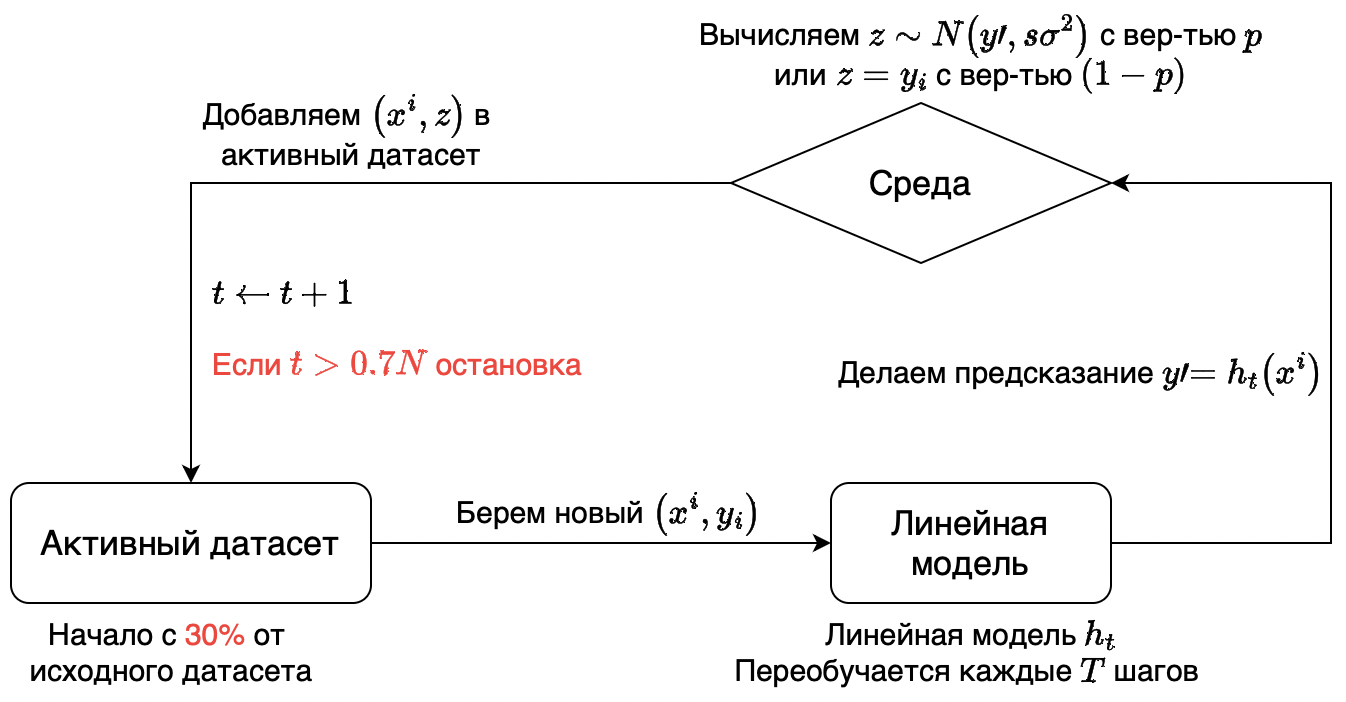
\includegraphics[width=0.47\linewidth]{pictures/Sliding window.png}
            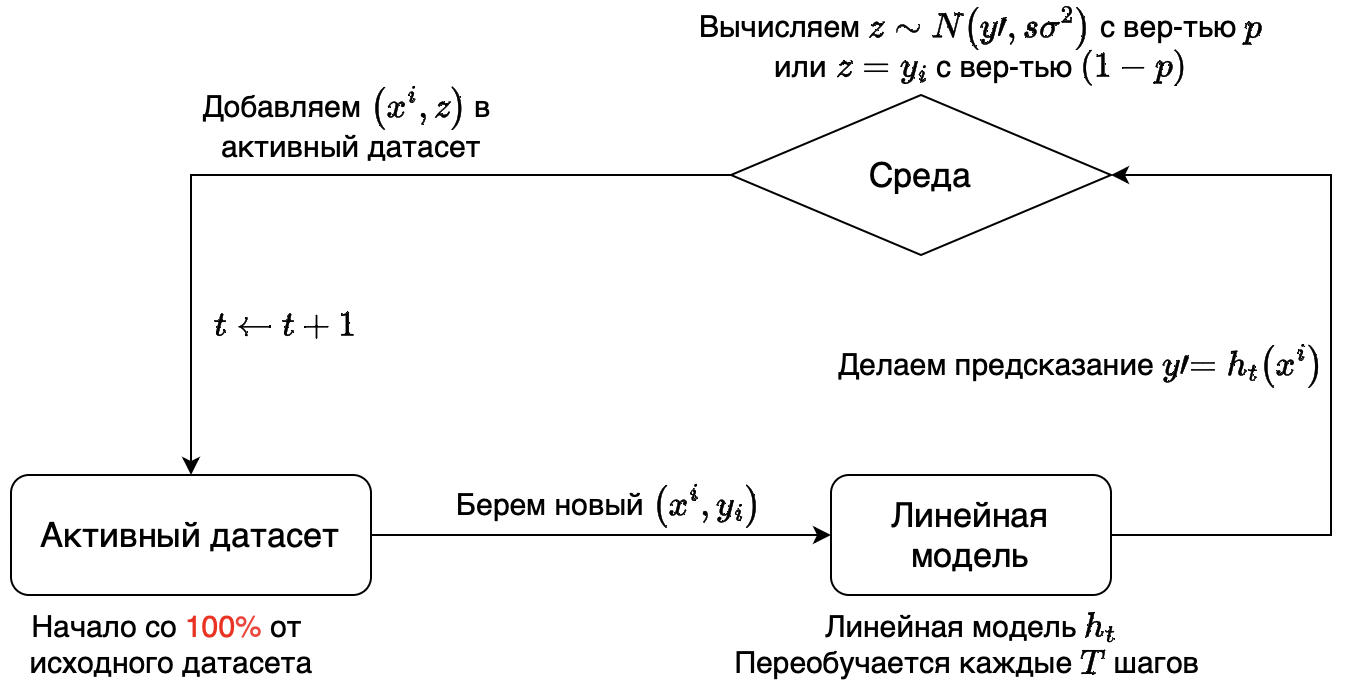
\includegraphics[width=0.47\linewidth]{pictures/Sampling update.png}
            \vspace{-2mm}
            \caption{\footnotesize{Две различные постановки эксперимента. Скользящее окно (слева) и обновление выборки (справа).}}
            \label{exp}
        \end{figure}

    \end{frame}
    
\section{Математическая модель эффекта обратной связи}
    \begin{frame}{Постановка задачи и теорема о предельном множестве}
        \footnotesize
        \vspace{-2mm}
        Определим следующую дискретную динамическую систему:
        \begin{equation}
            \label{system}
            f_{t+1}(x) = \text{D}_t(f_t)(x) ~ \text{ для } ~ \forall x \in \mathbb{R}^n, t \in \mathbb{N} ~\text{ и } ~ \text{D}_t \in \mathbb{D},
        \end{equation}
        где $\text{D}_t$ обычно называется оператором эволюции, $f_t(x)$ -- функции плотности вероятности распределения данных системы, а начальная функция $f_0(x)$ задана. 
        \vspace{-2mm}
        \begin{theorem_rus}[Veprikov et al., 2024] \label{delta}
        \vspace{-3mm}
            Для любой функции плотности $f_0(x), x \in \mathbb{R}^n$ и дискретной динамической системы \eqref{system}, если существуют $ g(x) \in L_1\left(\mathbb{R}^n\right)$ и $\psi_t \geq 0$ такие, что $f_t\left(x\right) \leq \psi_t^n \cdot |g(\psi_t \cdot x)|$ для всех $t \in \mathbb{N}$ и $x \in \mathbb{R}^n$.

            Тогда, если $\psi_t$ расходится к $\infty$, плотности $f_t(x)$ стремятся к дельта-функции, $f_t(x) \underset{t \to +\infty}{\longrightarrow} \delta(x)$ слабо.  

            Если $\psi_t$ сходится к нулю, тогда плотности $f_t(x)$ сходятся к нулевому распределению, $f_t(x) \underset{t \to +\infty}{\longrightarrow} \zeta(x)$ слабо.
        \end{theorem_rus}
        Для задачи регрессии, когда данные имеют вид $(X, y)$ Теорема \ref{delta} записывается не для данных в системе, а для случайного вектора невязок модели $h$, вида $y - h(X)$.
        
        Из Теоремы \ref{delta} можно вывести вид огибающих отображений $\text{D}_{\overline{1, t}}(\cdot) := \text{D}_t(\text{D}_{t-1} ( ... \text{D}_1( \cdot ) ... ))$, которые имеют вид
        \begin{equation} \label{cool_D}
            \text{D}_{\overline{1, t}}(f_0)(x) = \psi_t^n \cdot f_0(\psi_t \cdot x) \quad \forall x \in \mathbb{R}^n \text{ и } \forall t \in \mathbb{N}.
        \end{equation}
        Если операторы эволюции системы \eqref{system} имеют вид \eqref{cool_D}, можно записать формулу для вычисления $\psi_t$:
        \begin{equation}
            \psi_t \simeq f_t(0) .
        \end{equation}
        
    \end{frame}
    
    \begin{frame}{Анализ условий существования петель обратной связи и автономности системы \eqref{system}}
    \footnotesize
        \vspace{-1mm}
        Предположение 1, сформулированное в [1], гласит, что в системе \eqref{system} существует петля положительной обратной связи, если оператор $\text{D}_t$ является сжимающим в метрическом пространстве предсказаний модели.
        \vspace{-2mm}
        \begin{lemma_rus}[Veprikov et al., 2024] \label{moments}
        \vspace{-3mm}
            Если система \eqref{system} с $n=1$ удовлетворяет условиям Теоремы~\ref{delta} и $\psi_t \to \infty$, тогда все $2k$-тые моменты невязок 
            $y - h(X)$ убывают со скоростью как минимум $\psi_t^{-2k}$.
    
            Если оператор эволюции системы \eqref{system} удовлетворяет \eqref{cool_D}, тогда все (не только четные) моменты 
            $y - h(X)$ убывают со скоростью $\psi_t^{-k}$.
    
            Если существует $q \in [1; +\infty]$ такой, что $\{\nu_k^0\}_{k=1}^{+\infty} \in l_q$ и оператор эволюции системы \eqref{system} удовлетворяет \eqref{cool_D}, тогда $\{\nu_k^t\}_{k=1}^{+\infty} \in l_1$ и $\{\nu_k^t\}_{k=1}^{+\infty} \underset{t \to \infty}{\overset{l_1}{\longrightarrow}} 0$.
        \end{lemma_rus}
        Из Теоремы~\ref{delta} следует, что существует специальный вид отображений \eqref{cool_D}, для таких отображений можно вывести критерий автономности системы \eqref{system}.
        \vspace{-2mm}
        \begin{theorem_rus}[Veprikov et al., 2024] \label{semigroup}
        \vspace{-3mm}
            Если операторы эволюции $\text{D}_t$ динамической системы \eqref{system} имеют вид \eqref{cool_D}, тогда система \eqref{system} автономна тогда и только когда, когда
            \begin{equation} \label{cond_semigroup}
                \psi_{\tau + \kappa} = \psi_{\tau} \cdot \psi_{\kappa} ~\forall \tau, \kappa \in \mathbb{N}.
            \end{equation}
        \end{theorem_rus}
        
    \end{frame}
    
    \begin{frame}{Сохранение предельного множества при преобразовании признаков}
        \footnotesize
        Анализируется оператор $G$, осуществляющий преобразование $(X, y) \overset{G}{\to} (X', y')$ пространства признаков $X$ и целевой переменной $y$ для модели машинного обучения в задаче обучения с учителем. 
        %Целью данного раздела является нахождение достаточных условий, при которых предельное распределение для системы невязок, полученное с помощью Теоремы \ref{delta}, сохраняется при преобразовании $(X, y) \to G(X, y)$.  
        \vspace{-2mm}
        \begin{lemma_rus}[Веприков и др., 2023]
        \label{lemma_1}
        \vspace{-2mm}
            %Пусть в системе \eqref{system} для задачи обучения с учителем и $L(y, h, Z)$ – функция потерь модели $h$, а $(Z_t, y_t)$ – выборка на шаге $t$, $(Z'_t, y'_t) = G(Z_t, y_t)$ – выборка после применения оператора $G$. 
            \begin{enumerate}
                \item  
                Eсли $\exists~ T \in \mathbb{N} : $ для $\forall t \geq T$ выполнено $L(y_t, h_t, X_t) \geq L(y'_t, h'_t, X'_t)$ и функции плотности $y_t-h_t(X_t) \to \delta(x)$, то функции плотности $y'_t-h'_t(X'_t) \to \delta(x)$.
            
	           \item 
                Если же $\exists~ T \in \mathbb{N} : $ для $\forall t \geq T$ выполнено $L(y_t, h_t, X_t) \leq L(y'_t, h'_t, X'_t)$ и функции плотности $y_t-h_t(X_t) \to \zeta(x)$, то функции плотности $y'_t-h'_t(X'_t) \to \zeta(x)$.
           \end{enumerate}
        \end{lemma_rus}
        Квадратичная (MSE) и другие функции потерь, часто применяемые в задаче регрессии, могут быть разложены на составляющие смещения, разброса и неустранимого шума в данных: 
        $$L(y, h, X) = \text{Bias}^2(y, h, X) + \text{Var}(y, h, X) + \sigma^2.$$
        \vspace{-7mm}
        \begin{lemma_rus}[Веприков и др., 2023]
        \label{lemma_2}
        \vspace{-2mm}
            \begin{enumerate}
                \item Если $\exists~ T \in \mathbb{N} : $ для $\forall t \geq T$ преобразование $G$ уменьшает сумму смещения и разброса на шаге $t$, тогда $\forall t \geq T$ выполнено $L(y_t, h_t, X_t) \geq L(y'_t, h'_t, X'_t).$

                \item Если же $\exists~ T \in \mathbb{N} : $ для $\forall t \geq T$ преобразование $G$ увеличивает сумму смещения и разброса на шаге $t$, тогда $\forall t \geq T$ выполненно $L(y_t, h_t, X_t) \leq L(y'_t, h'_t, X'_t).$
            \end{enumerate}
        \end{lemma_rus}

    \end{frame}

\section{Эксперименты}
    \begin{frame}{Предел к дельта-функции или нулевому распределению}
    \footnotesize
    \vspace{-2mm}
        \begin{figure}
            \centering
            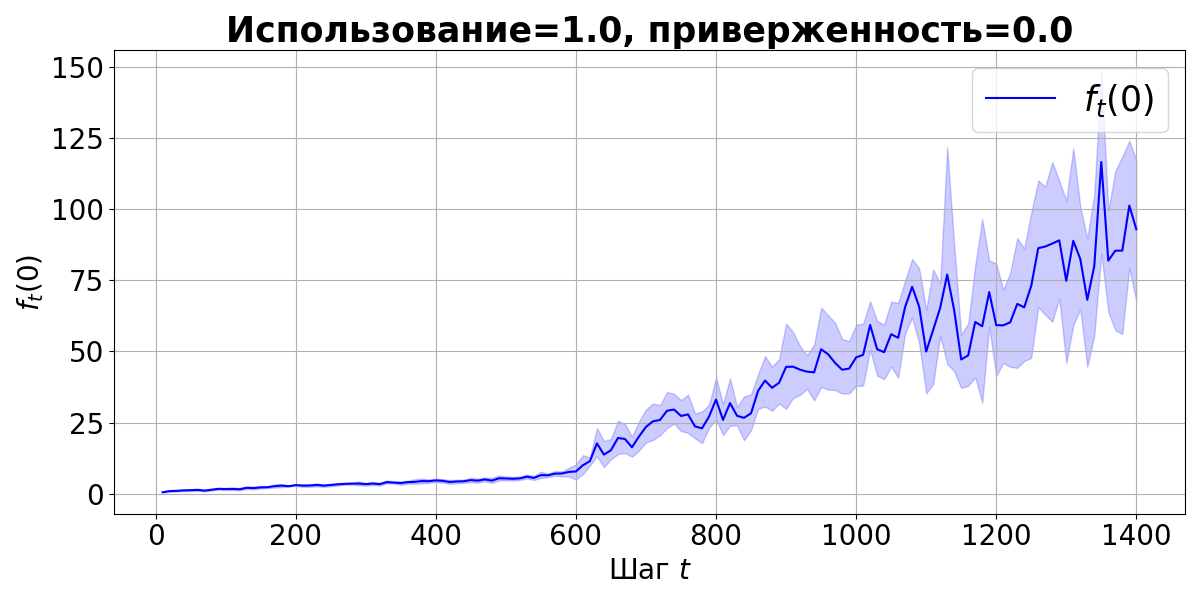
\includegraphics[width=0.45\linewidth]{pictures/ft0_sw_synthetic_sgd_model_50_1.0_0.0.png}~
            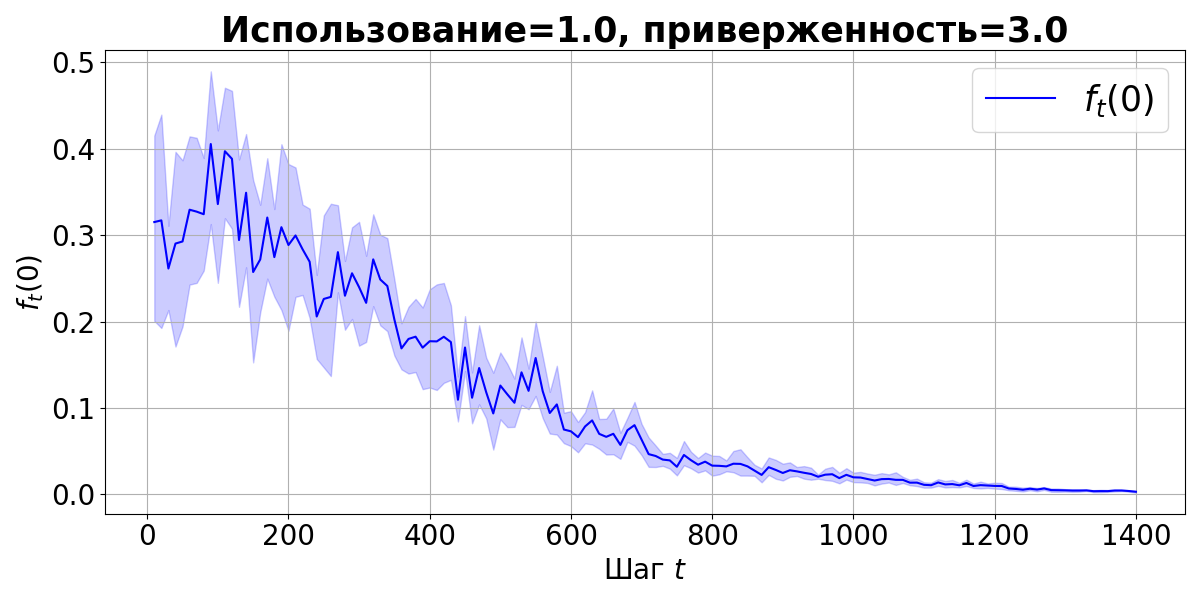
\includegraphics[width=0.45\linewidth]{pictures/ft0_sw_synthetic_sgd_model_50_1.0_3.0.png}

            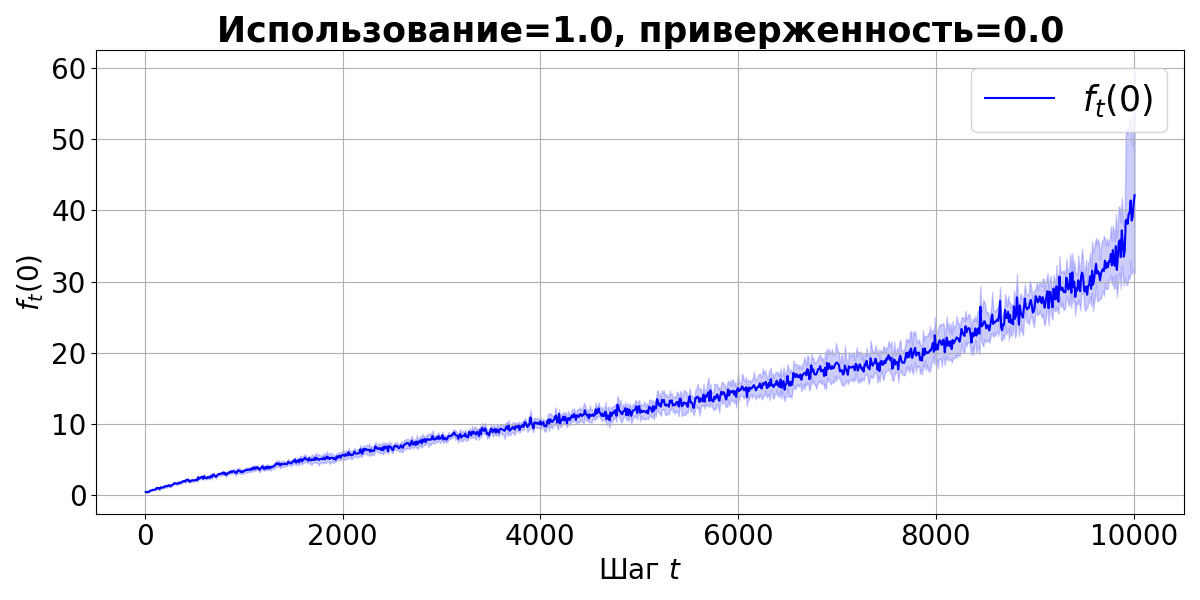
\includegraphics[width=0.45\linewidth]{pictures/ft0_su_synthetic_sgd_model_50_1.0_0.0.png}~
            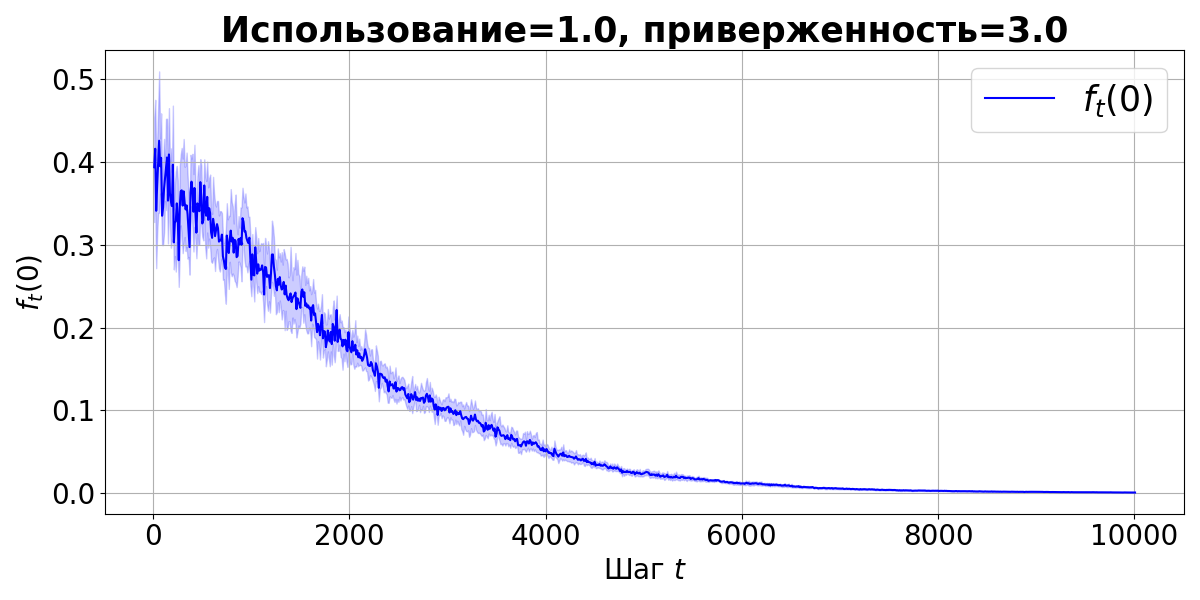
\includegraphics[width=0.45\linewidth]{pictures/ft0_su_synthetic_sgd_model_50_1.0_3.0.png}
            \vspace{-4mm}
            \caption{Постановка скользящее окно (сверху), обновление выборки (снизу).}
        \end{figure}
    \end{frame}

    \begin{frame}{Стремление моментов к нулю и исследование систем на автономность}
    \footnotesize
    \vspace{-2mm}
        \begin{figure}
            \centering
            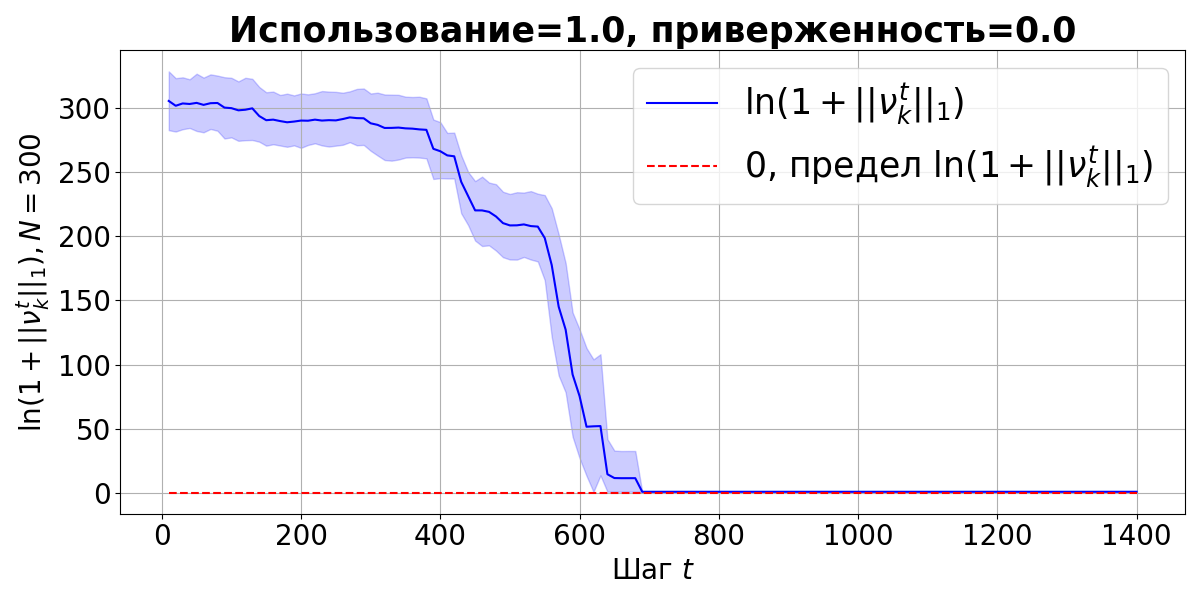
\includegraphics[width=0.473\linewidth]{pictures/k_mom_sw_synthetic_sgd_model_50_1.0_0.0.png}~
            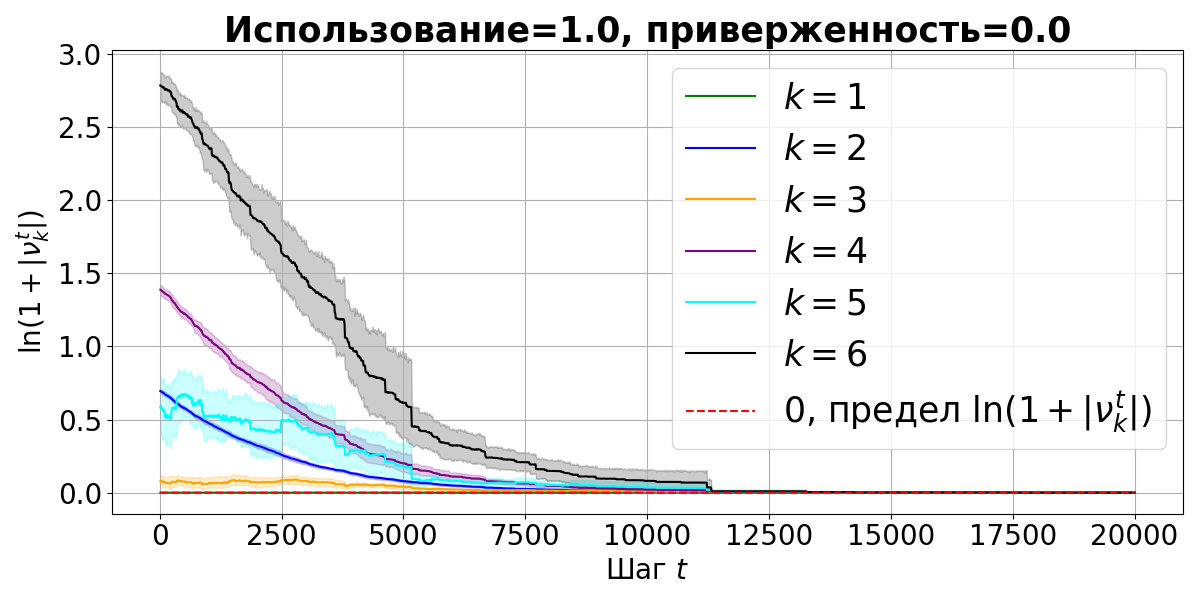
\includegraphics[width=0.473\linewidth]{pictures/k_mom_su_synthetic_sgd_model_50_1.0_0.0.png}
            
            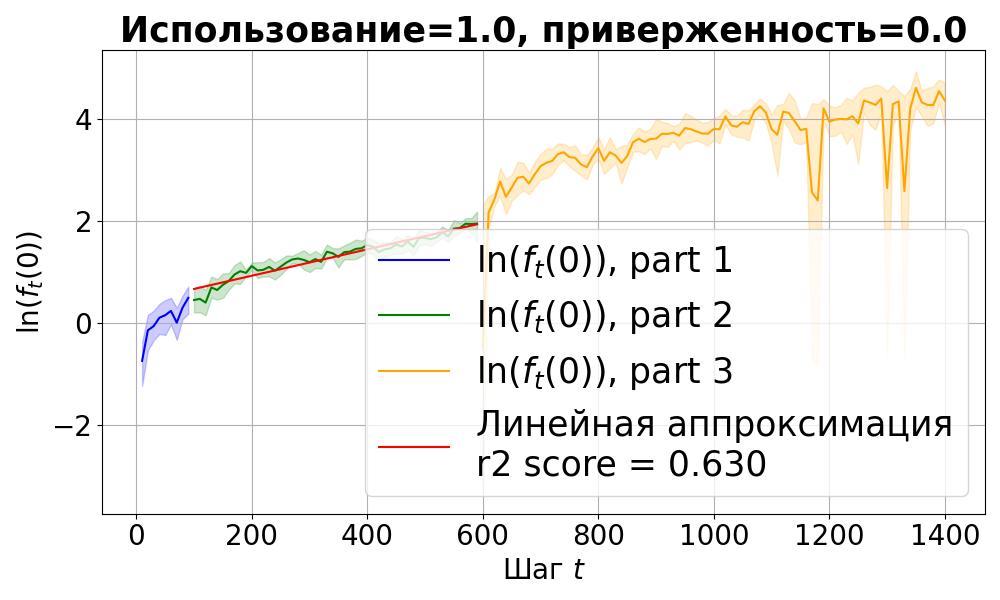
\includegraphics[width=0.32\linewidth]{pictures/aut_sw_synthetic_sgd_model_50_1.0_0.0.png}
            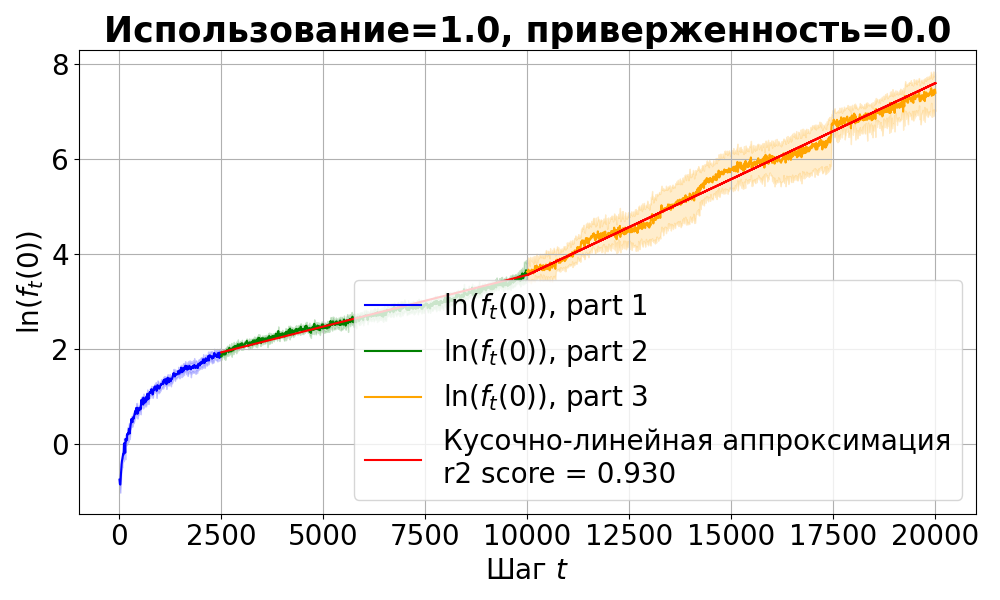
\includegraphics[width=0.32\linewidth]{pictures/aut_su_synthetic_sgd_model_50_1.0_0.0.png}
            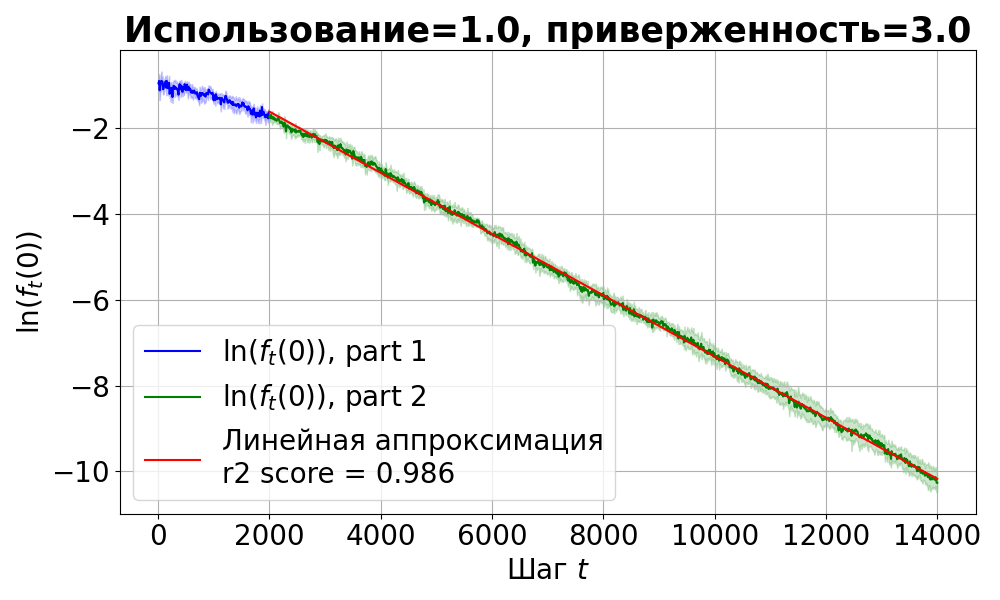
\includegraphics[width=0.32\linewidth]{pictures/aut_su_synthetic_sgd_model_50_1.0_3.0.png}
            \vspace{-5mm}
            \caption{Стремление моментов к нулю(сверху): скользящее окно(слева), обновление выборки(справа).
            \centering{Проверка автономности(снизу): скользящее окно(слева), обновление выборки(середина и справа).}}
        \end{figure}
    \end{frame}

    \begin{frame}{Сохранение предельного множества при преобразовании признаков}
        \footnotesize
        \vspace{-3mm}
        \begin{figure}
            \centering
            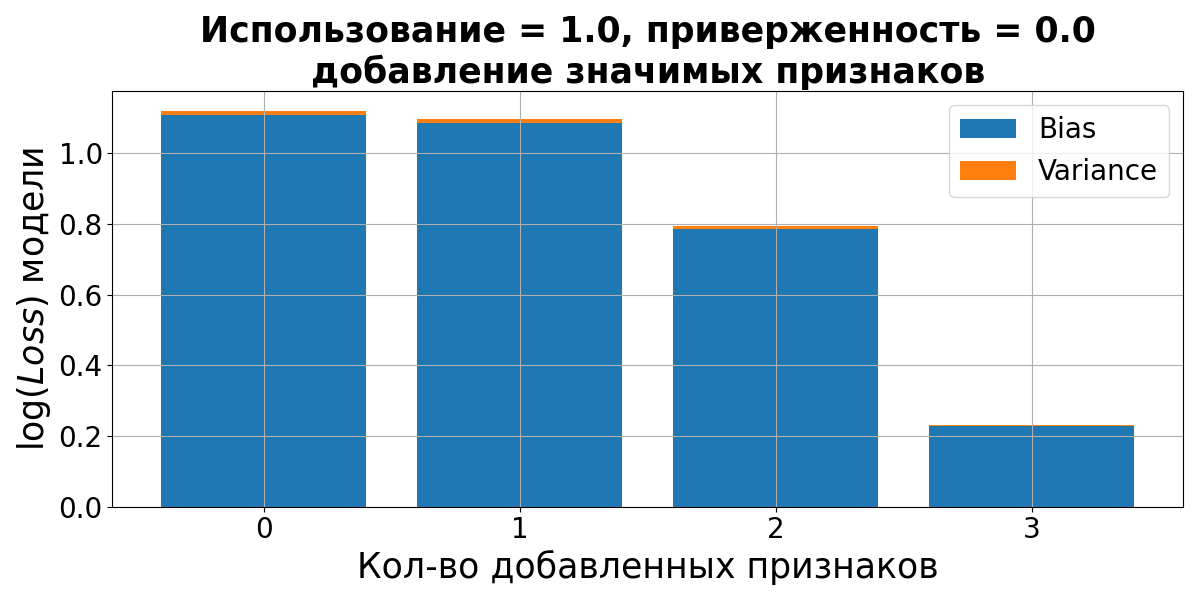
\includegraphics[width=0.45\linewidth]{pictures/conf_bvl_aif_1.0_0.0.png}~
            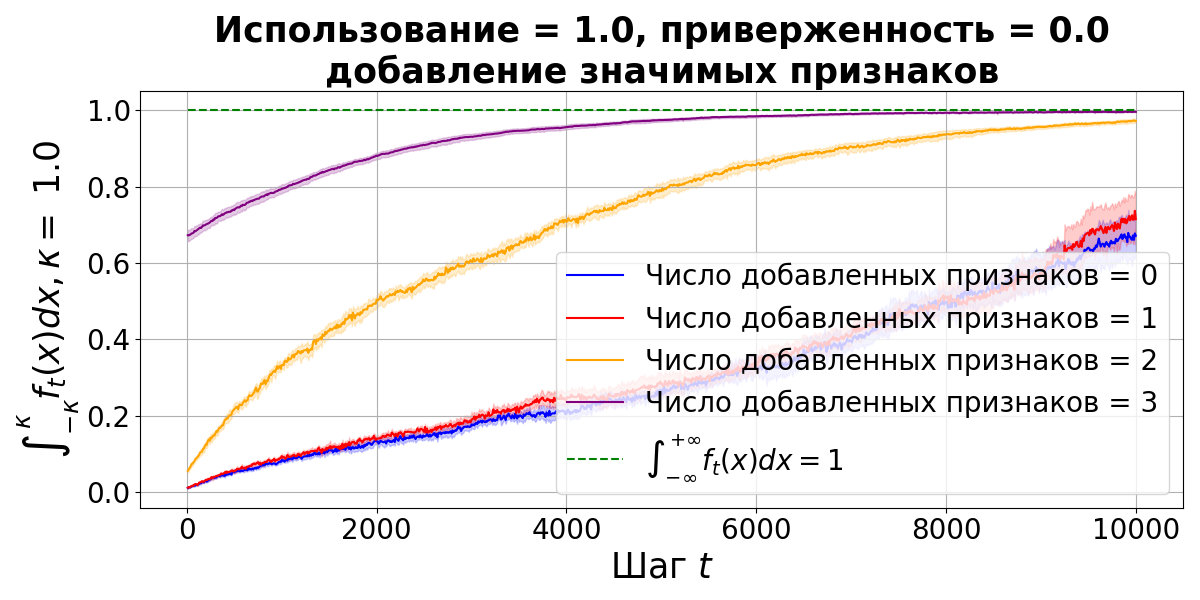
\includegraphics[width=0.45\linewidth]{pictures/conf_delta_aif_1.0_0.0.png}

            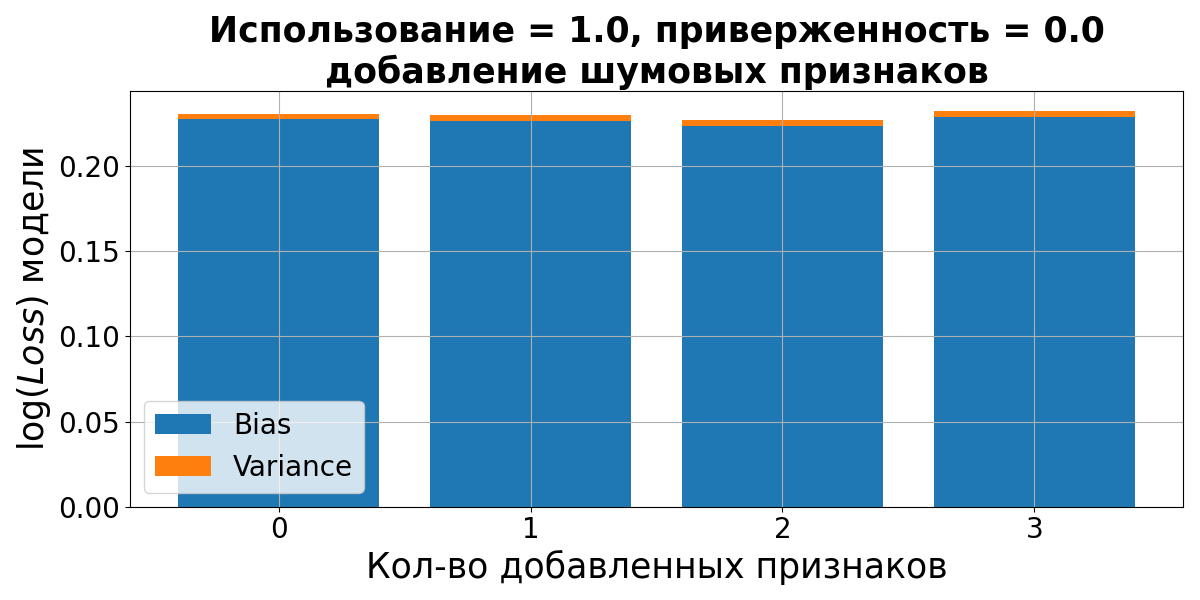
\includegraphics[width=0.45\linewidth]{pictures/conf_bvl_anf_1.0_0.0.png}~
            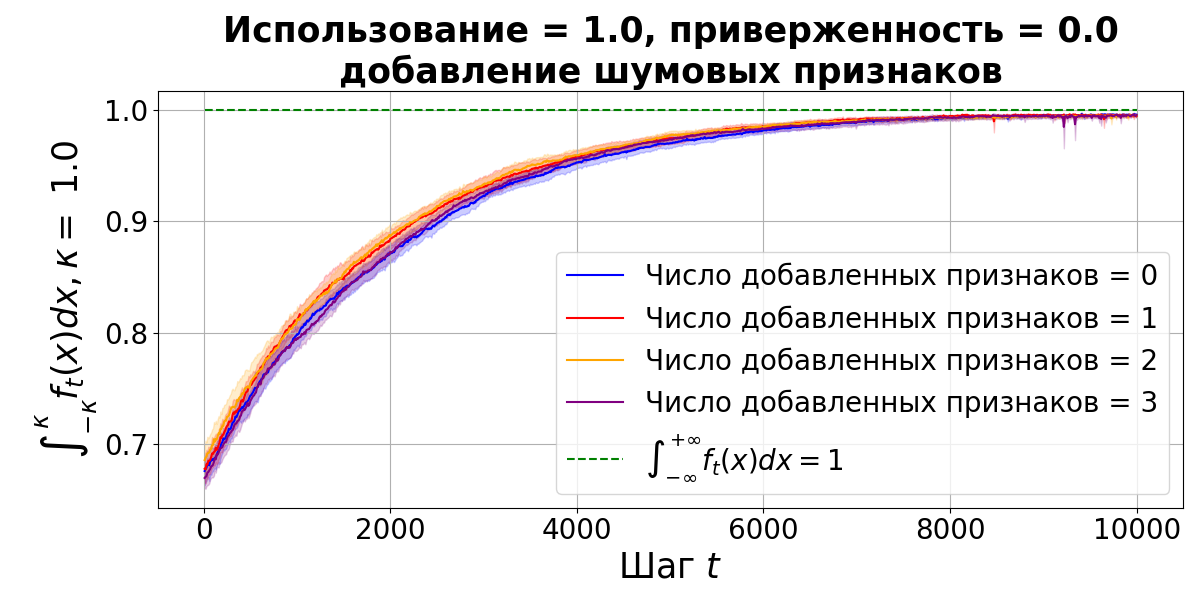
\includegraphics[width=0.45\linewidth]{pictures/conf_delta_anf_1.0_0.0.png}
            \vspace{-3mm}
            \caption{Добавление информативных (сверху) и неинформативных (снизу) признаков.}
        \end{figure}
    \end{frame}

\section{Вывод}
    
    \begin{frame}{Вывод}
        \begin{enumerate}
            \footnotesize
            \item В данной работе построена математическая модель эффекта петель обратной связи с использованием дискретных динамических систем

            \item Были получены результаты для определения предельного множества динамической системы, достаточных условий существования петли обратной связи, критерий автономности и достаточные условия сохранения предельного множества при преобразовании признаков

            \item В данной работе на языке Python разработан стенд проведения вычислительных экспериментов, симулирующий процесс многократного машинного обучения

            % \item Все полученные результаты строго доказаны и проверены в вычислительном эксперименте.
            
            \item Полученные результаты применимы для контроля качества систем ИИ в медицине, персонализации образования, широком классе СППР для выполнения требований кодекса этики в сфере ИИ и требований ГОСТ

            \item Мой вклад в данное исследование состоит в доказательстве теоретических исследований, участие в постановке экспериментов, сборе, обработке и анализе их результатов

            \item По результатам работы была подана статья в Q1 журнал (Veprikov et al., 2024), рассказано выступление на конференции ММРО-2023 (Веприков и др., 2023), материалы которой были поданы в журнал ИИПР
        \end{enumerate}

    \end{frame}

\section{Список литературы}
    \begin{frame}{Список литературы}
        \scriptsize

        \begin{enumerate}
            \item[1] \textcolor{myNewColorA}{(Veprikov et al., 2024)} Veprikov A.,   Afanasiev A., Khritankov A. A Mathematical Model of the Hidden Feedback Loop Effect in Machine Learning Systems // arXiv preprint \url{https://arxiv.org/abs/2405.02726}
            
            \item[2] \textcolor{myNewColorA}{(Веприков и др., 2023)} Веприков А. С., Афанасьев А. П., Хританков А.С. Математическая модель эффекта обратной связи в системах искусственного интеллекта // Сборник тезисов 21-й Всероссийской конференции Математические методы распознавания образов (ММРО-21). – Российская академия наук, 2023. – С. 35-37 
            
            \item[3] \textcolor{myNewColorA}{(Khritankov, 2023)} Khritankov A. Hidden feedback loops in machine learning systems: A simulation model and preliminary results // Software Quality: Future Perspectives on Software Engineering Quality: 13th International Conference, SWQD 2021, Vienna, Austria, January 19–21, 2021, Proceedings 13. – Springer International Publishing, 2021. – С. 54-65.

            %\item \textcolor{myNewColorA}{(Khritankov, 2023b)} Khritankov A. Positive feedback loops lead to concept drift in machine learning systems // Applied Intelligence. – 2023. – Т. 53. – №. 19. – С. 22648-22666. 
            
            \item[4] \textcolor{myNewColorA}{(Taori et al., 2023)} Taori R., Hashimoto T. Data feedback loops: Model-driven amplification of dataset biases // International Conference on Machine Learning. – PMLR, 2023. – С. 33883-33920.
            
            \item[5] \textcolor{myNewColorA}{(Adam et al., 2022)} Adam G. A. et al. Error amplification when updating deployed machine learning models // Machine Learning for Healthcare Conference. – PMLR, 2022. – С. 715-740.

            \item[6] \textcolor{myNewColorA}{(Terren et al., 2021)} Terren L. T. L., Borge-Bravo R. B. B. R. Echo chambers on social media: A systematic review of the literature // Review of Communication Research. – 2021. – Т. 9.

            \item[7] \textcolor{myNewColorA}{(Mansoury et al., 2020)} Mansoury M. et al. Feedback loop and bias amplification in recommender systems //Proceedings of the 29th ACM international conference on information and knowledge management. – 2020. – С. 2145-2148.

            \item[8] \textcolor{myNewColorA}{(Davies et al., 2018)} Davies H. C. Redefining filter bubbles as (escapable) socio-technical recursion // Sociological Research Online. – 2018. – Т. 23. – №. 3. – С. 637-654.

        \end{enumerate}
    \end{frame}

\end{document}
